\documentclass{article}%
%\geometry{verbose,letterpaper,tmargin=2.54cm,bmargin=2.54cm,lmargin=2.54cm,rmargin=2.54cm}
\errorcontextlines=999
\usepackage{setspace}%
%\usepackage{subfigure}%
\usepackage{lineno}%
\usepackage{authblk}%
\usepackage[parfill]{parskip}
\usepackage{hyperref}
\usepackage[backend=biber,
natbib=true,
mincitenames = 1,
maxcitenames = 3,
uniquename = false,
uniquelist = false,
bibstyle = ele,
citestyle = authoryear-comp]{biblatex}%
\addbibresource{Stable_Isotopes_and_Fatty_acids.bib}%
\usepackage{mathtools}%
\usepackage{graphicx}%
\usepackage[position = top,labelformat=simple,font = bf]{subfig}

%\renewcommand*{\finalnamedelim}{\addspace\&\space}
%\captionsetup[subfloat]{justification=justified,singlelinecheck=false}

\makeatletter%
\def\@maketitle{%
  \vskip 2em%
  \begin{center}%
%  \let \footnote \thanks
    {\Large\bfseries \@title \par}%
    \vskip 1.5em%
    {\normalsize
      \lineskip .5em%
      \begin{tabular}[t]{c}%
        \@author
      \end{tabular}\par}%
    \vskip 1em%
    {\normalsize \@date}%
  \end{center}%
  \par
  \vskip 1.5em}
\makeatother

\begin{document}%

\begin{titlepage}%
\title{Bayesian estimation of predator diet composition from fatty
  acids and stable isotopes}%
\renewcommand\footnotemark{}

\author{Philipp Neubauer*}\thanks{*Corresponding author electronic address: neubauer.phil@gmail.com}%
\affil{Dragonfly Science,\\PO Box 27535, Wellington 6141, New Zealand}%

\author{Olaf P. Jensen}%
\affil{Institute of Marine and Coastal Sciences\\Rutgers University, New Brunswick, NJ 08901, USA}%

\date{Dated: \today}%

\maketitle%

\end{titlepage}

 \begin{spacing}{1.9} 
 \begin{flushleft}

\setcounter{page}{1}
\linenumbers
\begin{abstract}
Quantitative analysis of stable isotopes (SI) and, more recently,
fatty acid profiles (FAP) are useful and complementary tools for
estimating the relative contribution of different prey items in the
diet of a predator. The combination of these two approaches, however,
has thus far been limited and qualitative. We propose a mixing model
for FAP that follows the Bayesian machinery employed in
state-of-the-art mixing models for SI. This framework provides both
point estimates and probability distributions for individual and
population level diet proportions. Where fat content and conversion
coefficients are available, they can be used to improve diet
estimates. This model can be explicitly integrated with analogous
models for SI to increase resolution and clarify predator-prey
relationships. We apply our model to simulated data, demonstrating feasibility and model
performance, and re-analyse an experimental dataset to illustrate modeling strategies
and applications to real fatty acid profiles. Our methods are provided as an open
source software package for the statistical computing environment R.
\end{abstract}

\textbf{Keywords} Stable isotope analysis, quantitative fatty acid analysis,
QFASA, lipid profile, diet analysis, Bayesian mixing model, fatty acid
signature, dietary marker

\section{Introduction}
Quantitative estimates of an animal’s diet are a critical component of
predator-prey studies, ecosystem models, and ecosystem-based
management. Existing methods of estimating diet proportions all have
strengths and weaknesses \citep{bowen_methods_2012}. Traditional
stomach content and fecal matter analysis represent a brief snapshot
of diet at a particularly place and time and can be invasive,
time-consuming, and potentially biased by differential rates of
digestion of prey or ingestion of identifiable prey parts
\citep{bowen_methods_2012}. Chemical markers such as stable isotopes
(SI) and fatty acid profiles (FAP) solve some of these problems.  For
example, both approaches integrate diet composition over an extended
time period -  typically weeks to months, depending on tissue turnover
rates  \citep{tucker_convergence_2008}. These advantages have led to rapid
growth in the use of chemical markers in diet studies
 \citep{elsdon_unraveling_2010,williams_using_2010,kelly_fatty_2011,
bowen_methods_2012}. However, chemical dietary markers generally lack
the specificity of traditional stomach content analysis. In
particular, several prey species often have similar isotopic signatures. More
recent studies have sought greater dietary resolution through the use
of SI of other elements in addition to carbon and
nitrogen \citep[e.g.,][]{belicka_stable_2012}, compound specific SI ratios
\citep[e.g.,][]{budge_tracing_2008,jack_individual_2011}, or a combination of stomach
content analysis and SI or FAP \citep[e.g.,][]{pethybridge_seasonal_2012}. The
use of SI and FAP in combination also holds great promise; however, studies that have used both chemical markers have been
qualitative \citep{[e.g.,][]guest_trophic_2009} or based on positive correlation
of results from both methods \citep{tucker_convergence_2008}.

Analysis tools for SI data have become very sophisticated in recent
years, starting with the development of general Bayesian analysis
tools for estimating diet proportions, and leading to customized
(hierarchical) models for individual applications \citep{moore_incorporating_2008,hopkins_estimating_2012,parnell_bayesian_2012}. The latter models
can, for instance, estimate dietary differences of geographically
distinct populations \citep{semmens_quantifying_2009}, accommodate temporal
changes in diets or estimate the effect of covariates (e.g., age,
size, sex) on diet proportions \citep{parnell_bayesian_2012}.While these
models provide a considerable step towards ecologically relevant
models in diet studies, the underlying SI data is limited in the
resolution that it can provide. Since typically only 2-3 SI are
measured, the contrast that is achievable from such a low number of
variables is necessarily limited, especially when the number of
potential prey items increases \citep{phillips_source_2003,ward_quantitative_2011}. Optimally aggregating prey items into prey groups may
circumvent this problem \citep{ward_quantitative_2011}, but may also be less
satisfactory in complex food webs.

FAP data can, in theory, provide considerably more resolution compared
to SI data, due to large number of potential fatty acids (FAs) that can be
measured. Furthermore, \citet{blanchard_inference_2011} developed a
Bayesian model for diet inference from FAs (furthering the
development of Bayesian mixing models for compositional data by
\citet{billheimer_compositional_2001}), showing that model based
inferences of predator diets from FAs are
achievable. Nevertheless, studies employing FAP remain either qualitative
in their estimates of prey proportions in predator diets, or use
Quantitative Fatty Acid Signature Analysis \citep[QFASA; ][]{iverson_quantitative_2004} to
obtain quantitative estimates of diet proportions. 

QFASA is the only available (i.e., off the shelf) method thus far for use with FAP data, and, in
contrast to recent (Bayesian) SI and FAP mixing models, relies on a distance
metric rather than a model based formulation to estimate the most
likely diet proportions. This framework provided the first
quantitative approach to estimating diet proportions using FAs
and it has already seen widespread use, particularly in studies of
marine mammals \citep{bowen_methods_2012} and seabirds
\citep{williams_using_2010}. Nevertheless, QFASA has a number of
limitations. Since it is not based on a probabilistic model, it is
difficult to estimate uncertainty associated with estimated diet
proportions \citep[but see Steward 2005 as cited in][]{blanchard_inference_2011}. The absence of an explicit model
also makes it impossible to build ecological mechanisms (e.g.,
covariates of consumed diets) directly into the model. Furthermore,
uncertainty about conversion coefficients representing enrichment and
preferential uptake of FAs cannot be considered, yet small
changes in these coefficients can lead to differences in inferred diet
proportions \citep{wang_validating_2010}.

Given the discrepancy in methods applied to SI and FAP data, it is
perhaps not surprising that their joint application has commonly
relied on qualitative comparisons. Because both markers integrate diet
composition over often comparable time-scales, however, an explicit
integration of these data types could provide substantial
benefits. While FAP data could mitigate the resolution problem in SI
data, SI data could provide increased resolution and clarify
predator-prey relationships, the knowledge of which is usually a
pre-requisite for FAP data. For example, for many non-modified fatty
acids, FAP alone cannot discriminate between the case of two species
which share a common diet and the situation in which one of these
species eats the other.  In either case, the two species may have
similar FAP. The addition of a stable isotope with trophic
fractionation (e.g., $^{15}N$), however, can readily distinguish predation
from dietary overlap.

Here, we develop a mixing model for FAP data based on a probabilistic
model whose parameters are estimated using Bayesian methods, and
explicitly integrate SI in the estimation of diet proportions. Using both simulated and
published data, we demonstrate the suitability of this model for FAP analysis and
highlight the potential benefit of explicit integration with SI data
to increase the precision of diet estimates.
 
\section{Methods}
\subsection{A Bayesian mixing model for fatty acid profiles}

Bayesian models for SI data are commonly based on the assumption that
SI ratios are normally distributed. This assumption cannot be made for
FAP data, since for most methods of analysis, the concentration of
individual FAs is normalized to the total lipid content of the
sample. Thus, the FAP are a collection of proportions (referred to as
a composition), which lie between 0 and 1, and are constrained to sum
to 1. A common solution to this problem, however, is to consider
transformations that make the data approximately normal
\citep{budge_studying_2006}. To construct our model, we considered the
additive log ratio transformation \citep{aitchison_convex_1999},
also called alr transformation, such that

\begin{align}
y_{i,s} = alr(\phi_{i,s}) = log \left( \frac{\phi_{i,s,1...p-1}}{\phi_{i,s,p}} \right)
\end{align}

where $\phi_{i,s}$ is the $p$-variate fatty acid composition of individual
$i$ of prey species $s$, with a total of $n$ potential prey species
considered. Note that in the following we often drop the subscript for
FAs, e.g., $\phi_{i,s}$ and $y_{i,s}$ are thus $p$ and $p-1$
dimensional vectors, respectively. We assumed that the distribution of $y$ is
multivariate normal, with species specific mean $\mu_s$ and covariance matrix $\Sigma_s$,
or $y_{i,s} \sim N(\mu_s,\Sigma_s)$. A vaguely informative prior on
$\mu_s$ and $\Sigma_s$ allows for uncertainty in prey distributions to propagate to estimates of diet proportions \citep{ward_including_2010}.

Each predator $j$ consumes a proportion $\pi_j$ of each prey source, and
analogous to stable isotope mixing models, predator FAP are then a
linear combination of prey FAPs, normalized to sum to one. Since predators may selectively assimilate or metabolize FAs
\citep{iverson_quantitative_2004,budge_studying_2006,rosen_effects_2012},
we specify prey-specific conversion coefficients $\kappa_{s}
= \kappa_{s,1}...\kappa_{s,p}$ for each of the $p$ FAs \citep{rosen_effects_2012}. Furthermore,
the $n$ prey species likely have different fat content $\Phi$
that will affect the total amount of FAs assimilated from each
prey species by the
predator. The expected FAP of predator $\tau_j$ is then a linear combination of the prey
FAP, modified by conversion coefficients for each fatty acid $p$ and fat
content for each prey $i$:

\begin{align}
\label{eq:2}
t_j &\sim N(alr(\tau_{j}),\Sigma_{\tau})\\
\tau_{j} &= C \left\{ \sum_{s}^n  \left(\pi_{j,s} \Phi_{s} \right) \left(
    \kappa_{s} \otimes \phi_{j,s} \right) \right\}
\end{align}

Here, $C$ is the closure operation which normalizes the FAP to sum to
one and $\otimes$ is the outer (element wise) product. $\phi_{s,j}$ is
the FAP of prey items of species $s$ consumed by predator
$j$. Similarly to \citet{parnell_bayesian_2012},
we thus assumed that individual predators do not necessarily feed on
'average' prey items, but rather consume prey items with
signatures drawn from the estimated prey distribution. We
formulate predator signatures $t$ as draws from a normal distribution after
transformation. We further assumed that
$\Phi$ and $\kappa$ are log-normally and gamma
distributed, respectively, around known mean and variance values (estimated or
calculated from controlled diet experiments, see below). The
closure operation in \autoref{eq:2} (i.e., the sum-to-one constraint
on the FAP) leads to $\kappa$ being determined in terms of
relative uptake of FAs (i.e., up to a multiplicative
constant), and implicitly makes the multivariate prior distribution over all $\kappa$ a Dirichlet
distribution. The same logic applies to $\Phi$, and in both cases we
opted for formulations that can be readily parametrized from priors
studies or published values (e.g., sample means and variances from experiments).

The diet proportions $\pi$ of predators are the main focus of investigation
in diet studies. These may be modeled at the (statistical) population
level (thus dropping the subscript $j$ in \autoref{eq:2}) or at the
individual level, as suggested in \autoref{eq:2}. In the latter case,
individual predator FAP can be modeled as draws from a population
level distribution of predator diet proportions. Recent approaches to stable
isotope mixing have focused on transformations of the diet proportion
vector $\pi$ to get around the
problems associated with the compositional nature of the diet
proportions in such a hierarchical setup, and we follow this approach
in our model. The diet proportions are transformed using clr
transformations \citep{semmens_quantifying_2009}, such that the
support of is the real line rather than the interval [0;1], and we
then assume that $clr(\pi_j) \sim N(\Pi,\Sigma_{\Pi})$, where $\Pi$ is the
vector of mean (population level) diet proportions. It is
then possible to model diet proportions as function of
covariates, such as size, sex, or region \citep[i.e., in a regression
formulation,][]{parnell_bayesian_2012}. While this approach is appealing, it adds to computation time needed
to estimate model parameters, and correlates with generally slower convergence. We therefore use a vague Dirichlet prior
on the proportions when convenient (i.e., when we estimate only
population level parameters).

Depending on the amount of samples for prey and predators, it
may be necessary to use informative priors for $\Sigma_{s}$ and
$\Sigma_{\tau}$. Both were given inverse-Wishart priors, and since both are co-variances of transformed data, it is
not straightforward to formulate default priors for these parameters. We have found that in practice manual adjustment of these priors
is often needed to be able to achieve convergence and mixing
(efficient exploration of the posterior distribution by the sampling
algorithm) of the Markov Chain Monte Carlo (MCMC) employed to estimate
model parameters. This is especially true when there are few source and/or predator samples. The
package allows for high level adjustment of these parameters through
the specification of the order of magnitude of the diagonal of each
covariance matrix. 

\subsection{Joint diet estimation from FAP and SI}
There are at least three potential benefits of integrating FAP and SI
data: i) increased information to discriminate among sources, ii) the
potential of SI to resolve predator prey relationships due to trophic
enrichment of SI, and iii) the potential reduction in estimation error
due to a larger body of research on fractionation coefficients for stable
isotopes as opposed to conversion coefficients in FAP. Integrating the two complimentary types of data
in a single model to estimate diet proportions may thus considerably
improve estimates of diet proportions over estimation from either
data-source alone.

Our model for FAP is conceptually similar to recent models proposed for SI data, and
integration of FAP and SI data into a single model is straightforward
in the present setting. We assume that the vector of SI signatures of
sampled prey
items $q$ follow a multivariate normal distribution, such that
$y_{q,s}^{SI} \sim N(\mu_s^{SI},\Sigma_s^{SI})$, where the superscript
$SI$ denotes that these are stable isotope signatures. Predator SI
signatures are again a linear combination of prey SI, this time
modified by additive fractionation coefficients
$\gamma$. Fractionation may, in turn, depend on prey isotope concentrations
\citep{hussey_rescaling_2014,caut_variation_2009}. In our model, we
assume additive fractionation, and suggest that concentration
dependence is taken into account when specifying distributions for
prey and SI specific fractionation coefficients $\gamma_s$ (see
examples below). The expected SI signature for predator $r$ is then

\begin{align}
\label{eq:3}
t_{r}^{SI} &=  \sum_{s}^n  \pi_{r,s}  \left(y_{q,r} + \gamma_{s} \right) \\
clr(\pi_{r}) &\sim N(\Pi,\Sigma_{\Pi})\\
\gamma_{s,SI} &\sim N(\nu_{SI},\sigma_{SI})
\end{align}


Note that the different subscripts to the FAP model imply that there is no need to have SI and
FAP from the same prey or predator samples, as long as we can assume that the prey samples are drawn
from the same statistical population as those for FAP, and that individual diet proportions of
predators are drawn from the same population distribution of diet
proportions.

The exact formulation of the integration of SI and FAP depends on the
assumptions that one is comfortable with in a given setting: identical
dietary proportions may be appropriate if diets (and hence SI and FAP)
are thought to be stable, or if both chemical tracers are thought to
integrate over similar time-scales. If the time scales of these two
elements are thought to be different (e.g., for different tissue
types), individual diet proportions may be more
appropriate, and may be drawn from an overall population distribution
of diet proportions. 


An R \citep{R_core_2014}
package (called fastinR) implementing methods outlined here, along with simulated
examples and the analysis of
experimental data described further below, is available on the
open source repository github.com/philipp-neubauer/fastinR. Models
implemented in the package include the above-mentioned formulations
for population level diet estimates, individual diet
estimates  as well as linear model
(regression and ANOVA) formulations for diet proportions, all
available for SI and FAP individually or as combined models (see
below). Model parameters were estimated using MCMC methods
implemented in JAGS \citep{plummer_jags_2003}, called
from R through higher level functions in the
fastinR package that allow for data input,
 inspection and manipulation.

\subsection{Simulation studies}

We initially explored the feasibility and performance of our model setup in a
range of simulations, which are illustrated (including code) in supplemental information S1. Simulations were also used to explore sensitivities of inferred diet proportions to the source
configuration and diet evenness in a series of
simulation experiments. We hypothesized that estimated diet
proportions are sensitive to diet source separation in FAP space,
co-linearity in FAP space \citep{blanchard_inference_2011} and diet makeup (e.g., specialist versus 
generalist diets). Further details and simulation results can be found
in supplemental information S2.

\subsection{Selecting fatty acids for analysis: an ordination approach}

% are there other analysis methods?
A potentially large number of FAs are available from analysis methods
such as gas-chromatography. A common practice is to simply set a
threshold and keep the most abundant FA for analysis. This practice
may, however, discard potential useful information, and a more
judicious approach is to retain FAs based on the among diet source
variability that they explain. \citet{wang_validating_2010} used a
method by which they tested the QFASA method on a series of subsets to
determine the subset that gave the best accuracy. Although feasible, such
a method is prohibitive with fully Bayesian models, which can take a long
time to run with a realistic dataset.

Here, we propose a variable selection method based on constrained
ordination, which considers the contribution of individual fatty
acids to axes separating diet sources. Based on this contribution
relative to the overall separation, the user can choose FAs
that contribute most to source separation. This procedure is intended
to reduce computation time (and dimensionality) of the models,
while retaining as much accuracy in diet estimates as possible. Further details about the
procedure are given in supplemental information S3.


\subsection{Application: estimating predator diets in a controlled
  experiment}

To illustrate the potential of the models presented above, we analysed
data from an experimental study by
\citet{stowasser_experimental_2006}, which investigated changes in
squid FAP and SI as a function of diet treatments. The treatments consisted of
exclusive fish and crustacean diets, as well as switched and mixed
diets, with the former switching diets from fish (henceforth SF, n=4) to
crustacean (SC, n=5) after 15 days of the 30 day experiment. 

In order to apply our model, we first estimated conversion
coefficients of FAP and fractionation in SI, using squid from the 30
day diet treatments feeding exclusively crustacean and fish diets. The
model for estimation of SI fractionation followed the model in
\citet{hussey_rescaling_2014}, thus accounting for diet $\delta^{15}N$
and $\delta^{13}C$, and used their results as priors for fractionation
parameters for $\delta^{15}N$, and results from \citet{caut_variation_2009} to
construct priors for $\delta^{13}C$. Estimation of FA conversion coefficients used
 \eqref{eq:2} with proportions assumed known from feeding
 trials. Computational details on the estimation of conversion coefficients and
 fractionation are given in supplemental information S4.

In our diet analysis, we analyzed samples from the switched diet treatments, and
used both SI and FAP to investigate if our models allow us to infer diet
proportions in either treatments. We subset the data to use only
switched diet squid that were analysed for FAP and SI after at least
10 days under the respective treatment. We only had overlapping
SI and FAP for the SC treatment squid, and we therefore started by analyzing this treatment in isolation to
demonstrate that both SI and FAP can resolve diet proportions, and to
demonstrate the benefit of using the two tracers in a joint model. We
then analyzed the SF treatment squid, for which we only had 3 specimen with FAP
and 1 specimen with SI. The markers available for this treatment did
not overlap for any of the sampled squid. 

We lastly estimated individual diet proportions in the SC
treatment. To demonstrate how the model based approach to diet estimation can be
use to answer ecologically relevant questions about predator
diets, we also analyzed SF and SC treatment squid together in a linear model
setup that investigated treatment differences explicitly. The linear
model used treatment dummy variables to estimate individual intercepts
for each treatment and prey combination, and allows us to estimate,
conditional on the data and priors, whether squid in either one
treatment group consumed significantly more of any one prey type.

FAP analyses used data obtained by analyzing digestive glad tissue, which is thought to
rapidly assimilate dietary FAs in relatively unmodified
proportions relative to the original diet. SI were analyzed from
muscle tissue since we had more individuals sampled for SI from this tissue, which may be more prone to fractionation and slower
turnover than digestive glad tissue. In the original study, a total of
25 FAs were reported. Here, we selected FAs using ordination
methods described above. For estimation of model parameters, priors for
prey and predator specific variances were adjusted manually to give
reasonable behaviour in the MCMC algorithm. The analyses are detailed
in supplemental information S5.

\section{Results}

\subsection{Simulation studies}
Simulated test cases suggested that our model can estimate diet
proportions from both SI and FAP (supplemental information S1), with
accuracy depending mainly on source separation and diet evenness (supplemental information S2). For very
uneven diet proportions, such as in the feeding trials analyzed in the
squid example, we found the choice of posterior means as point estimate for diet
proportions inevitably introduced error at the margins of
the 0-1 interval when compared to true simulated diet
proportions.

Models with low accuracy conversion coefficients (with prior mean for
all FA set to 1 and large prior variance) also performed substantially
worse than models with accurately specified coefficients when
comparing point estimates of diet proportions to simulated diet
proportions (supplemental information S2), showing decreasing accuracy with increasing variance among simulated convergence coefficients.

\subsection{Squid diet experiments}

Dimension reduction by NMDS on FAP of squid and their potential prey suggested that crustacean diets were
readily distinguishable from fish diets
(\autoref{fig:squid_FAP}a). For fish diet items, however, no single
fish species could be clearly distinguished from any other fish species. Predator signatures of switched diet squid aligned with their
respective diets after correcting by posterior means of estimated conversion
coefficients. The latter were different from expected ($1/p$) for many
FA in the analysis (supplemental information S4).


\begin{figure}
  \begin{center}
      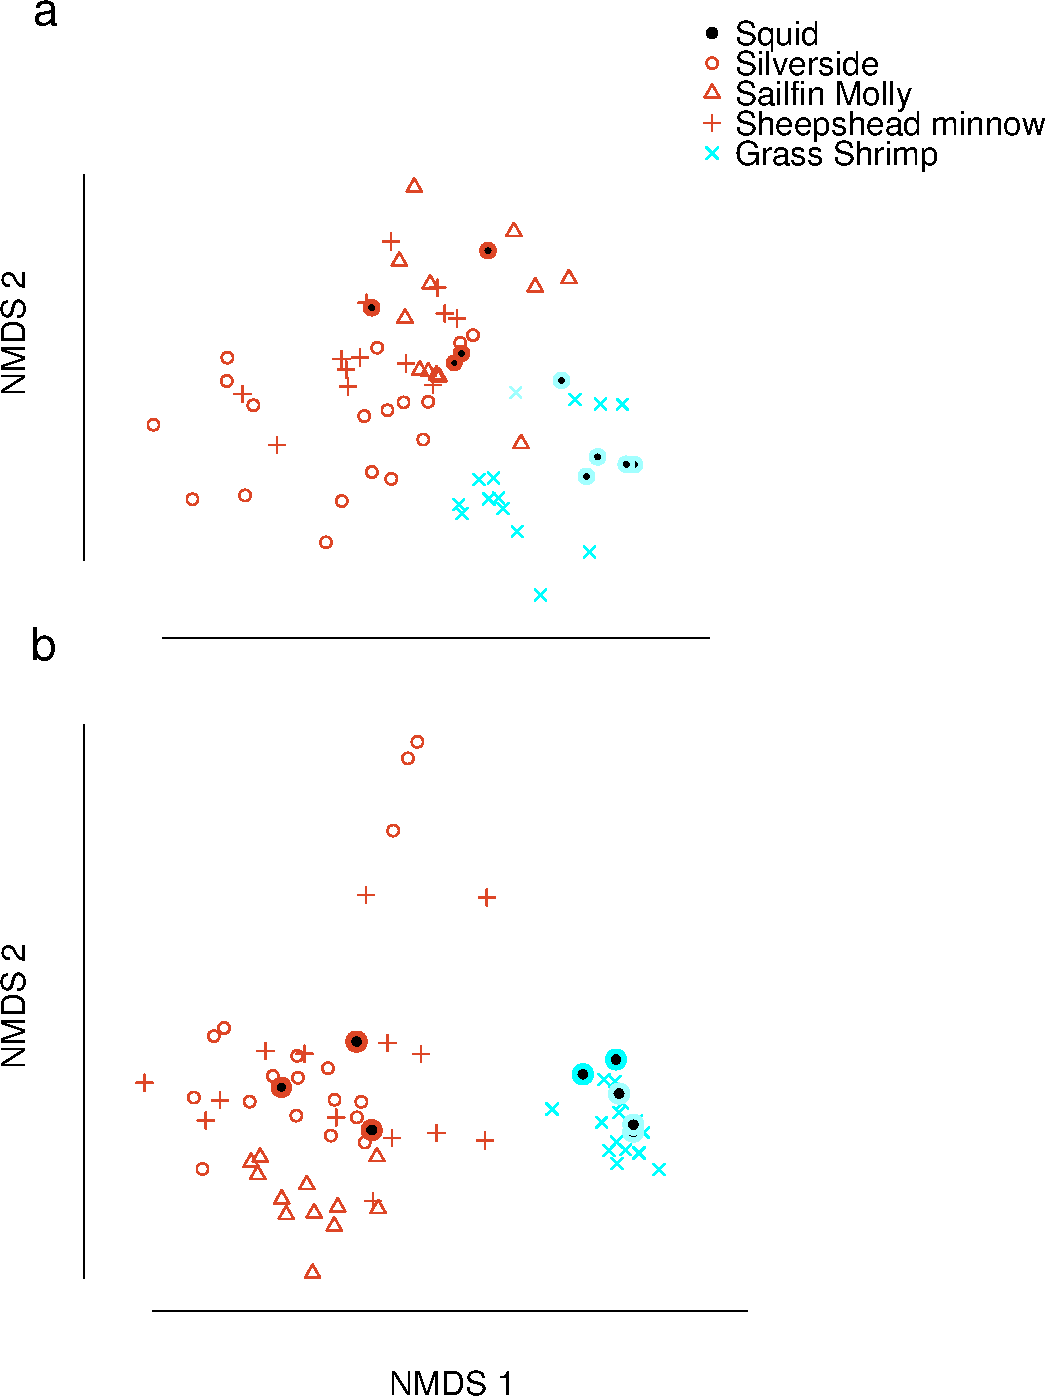
\includegraphics[width=0.75\textwidth]{figures/2nd_NMDS_pre.pdf}
    \caption{Non-metric Multi-Dimensional Scaling (NMDS) plots of FAP
      for 
      squid and their potential prey a) before and b) after variable selection.}
    \label{fig:squid_FAP}
  \end{center}
\end{figure}

Selection of FAs using constrained ordination
lead to four FAs, 22.6n.3, 20.5n.3, 20.4n.6 and 18.1n.9 being
retained for analysis (\autoref{fig:var_select}), accounting for a
total of 74\% of total among source variation on ordination axes
while maintaining a low prey matrix condition number ($\kappa=15.67$),
suggesting limited co-linearity. The matrix condition number nearly
doubled for the next most important fatty acid ($\kappa=29.17$) and
increased exponentially thereafter with addition of other FAs. The
resulting NMDS plot suggested that the reduction from 22 to four FA did
not significantly alter the configuration of predators and prey items
in FAP space, despite the drastically lowered number of input
dimensions (\autoref{fig:squid_FAP}b). Retaining a larger subset of
FAs (8 FAs) did not qualitatively alter the results, but did lead to lower
uncertainty in diet proportion estimates, suggesting that we lost some
relevant information by retaining only four of 25 original FAs to
reduce computational requirements.

\begin{figure}
  \begin{center}  
      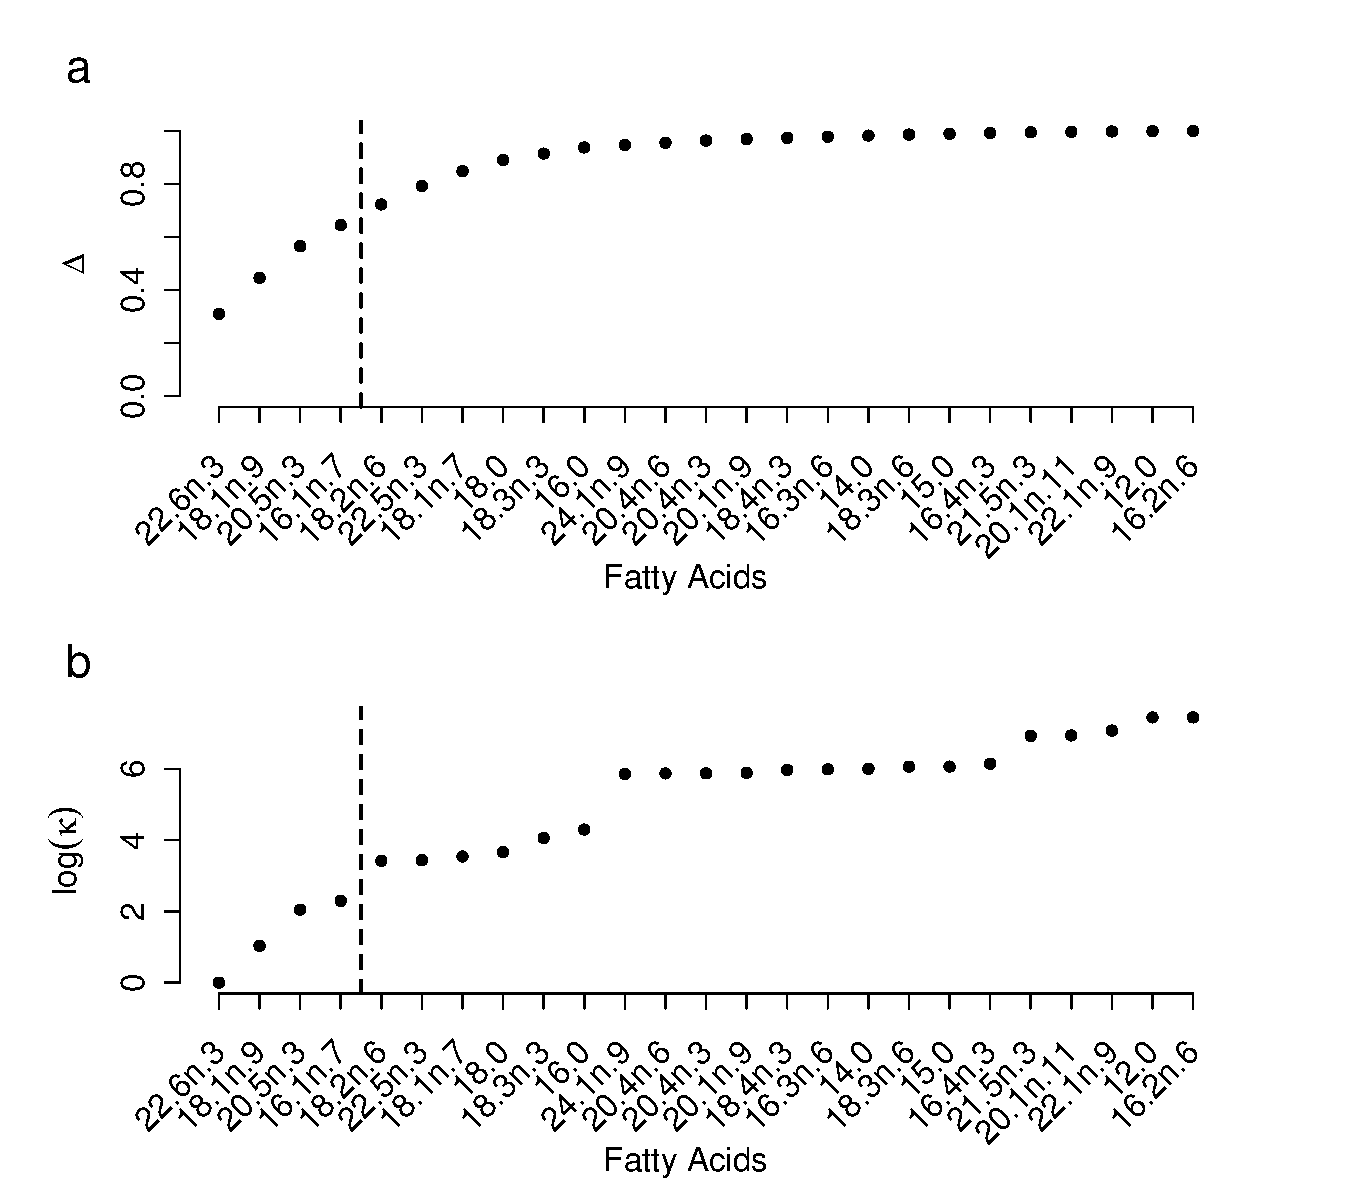
\includegraphics[width=0.75\textwidth]{figures/var_select.pdf}
      \caption{a) Cumulative proportion of between prey variance along CAP axes
      explained by individual fatty acids being added to the datasets,
      ordered by the contribution of each fatty acid to the total
      variance. b) Prey matrix condition number as a function of
      individual fatty acids being added as in a).}
    \label{fig:var_select}
  \end{center}
\end{figure}

SI also showed clear separation between crustacean and fish prey (\autoref{fig:squid_SI}),
but showed two groups for fish prey items, both consisting of specimen
from more than one fish species. Squid $\delta^{15}N$ was also substantially lower than any
of the prey species analysed even after correcting for estimated
fractionation coefficients.

\begin{figure}
  \begin{center}   
      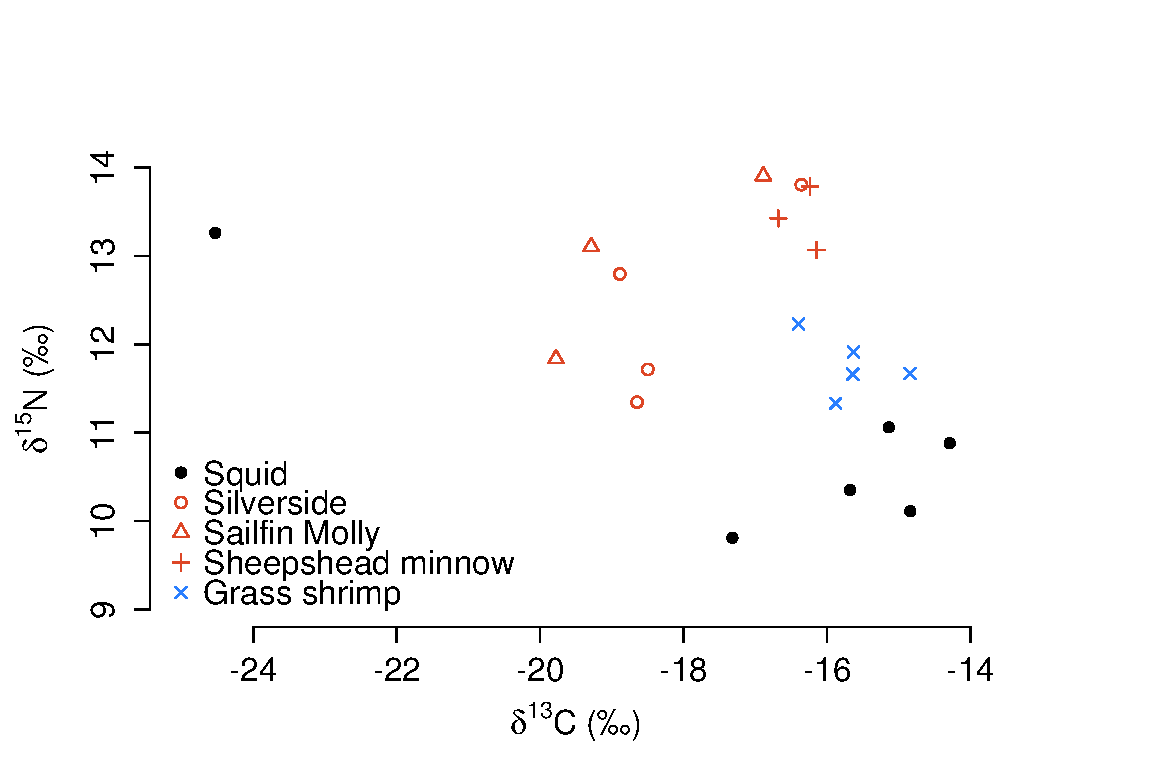
\includegraphics[width=0.75\textwidth]{figures/SI_plot.pdf}
       \caption{Stable isotope signatures of squid and their potential prey.}
    \label{fig:squid_SI}
  \end{center}
\end{figure}

FAP were able to resolve population level SC treatment squid diets,
suggesting a diet predominantly based on crustaceans
(\autoref{fig:pop_comp}). While uncertainty about the exact diet
proportions remained for both crustaceans and fish, most of the
posterior density for crustacean diet proportions was clearly
concentrated towards high
proportions of squid. For fish, posteriors were peaked near zero,
however, all fish species posteriors had long tails that spanned
nearly the whole interval of possible diet contributions. An analyses
based on SI alone gave very similar results, despite different tissue
types examined (\autoref{fig:pop_comp}). 

Combining the two markers lead to a substantial reduction in the
uncertainty of estimated diet proportions (\autoref{fig:pop_comp}),
and suggested a clear dominance of crustaceans in the diet. For the
combined analysis, the spread of the posterior distribution for crustaceans in the
squid diet was reduced by approximately 30\%, and most of the
probability density was shifted closer to one, and the reductions in
the spread of posterior distributions for fish diet items were as high
as 70\%. Lastly, estimates of individual diet proportions closely
mirrored population level estimates (\autoref{fig:ind_est}).

\begin{figure}
  \begin{center}
    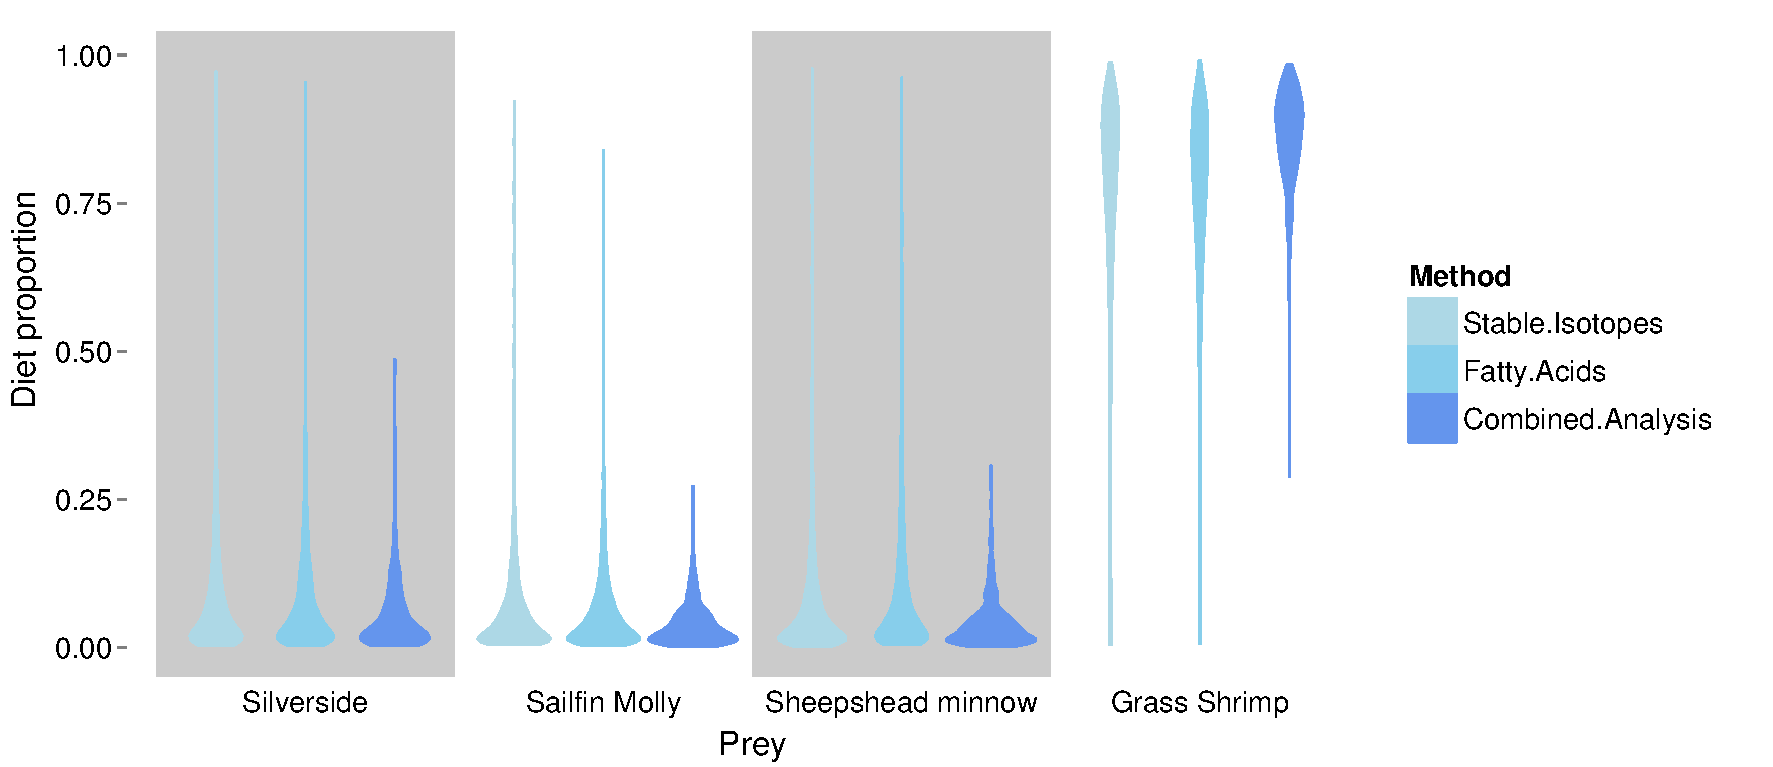
\includegraphics[width=1\textwidth]{figures/Comp_plot_violin.pdf}
    \caption{Posterior densities for diet proportion estimates of SC (crustacean only diet)
      treatment squid based on FAP, SI and a combined (FAP \& SI) analysis.}
    \label{fig:pop_comp}
  \end{center}
\end{figure}


\begin{figure}
  \begin{center}
    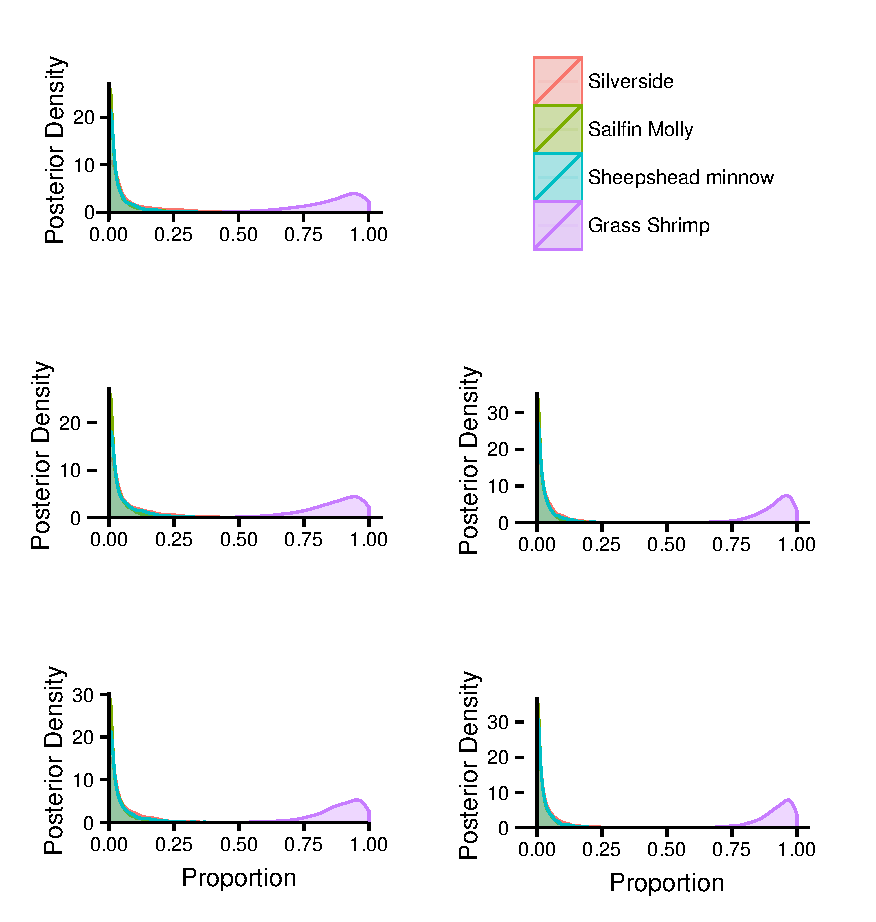
\includegraphics[width=0.8\textwidth]{figures/Ind_FAP_SC_long.pdf}   
    \caption{Posterior densities for individual diet proportion
      estimates of SC squid based on a hierarchical
      model for diet proportions using both FAP and SI.}
    \label{fig:ind_est}
  \end{center}
\end{figure}

Due to overlap of fish species in FAP and SI space, similar models for
SF treatment fish were unclear about the contribution of individual
fish species (\autoref{fig:pop_comp_SF}), but suggested that
crustaceans were a small part in the diet of these squid. SI and FAP
combined (i.e., adding one squid with SI but no FAP data) did not
provide much improvement for individual fish species, and the linear model setup was unable to identify significant differences
between diet proportions of individual prey items in the two
treatments due to uncertainty about individual fish species'
contributions (supplemental information 5). However, combining fish species post-hoc as the sum of individual posterior
distributions clearly shows a fish based diet
(\autoref{fig:Fish_plot}). 

\begin{figure}
  \begin{center}
    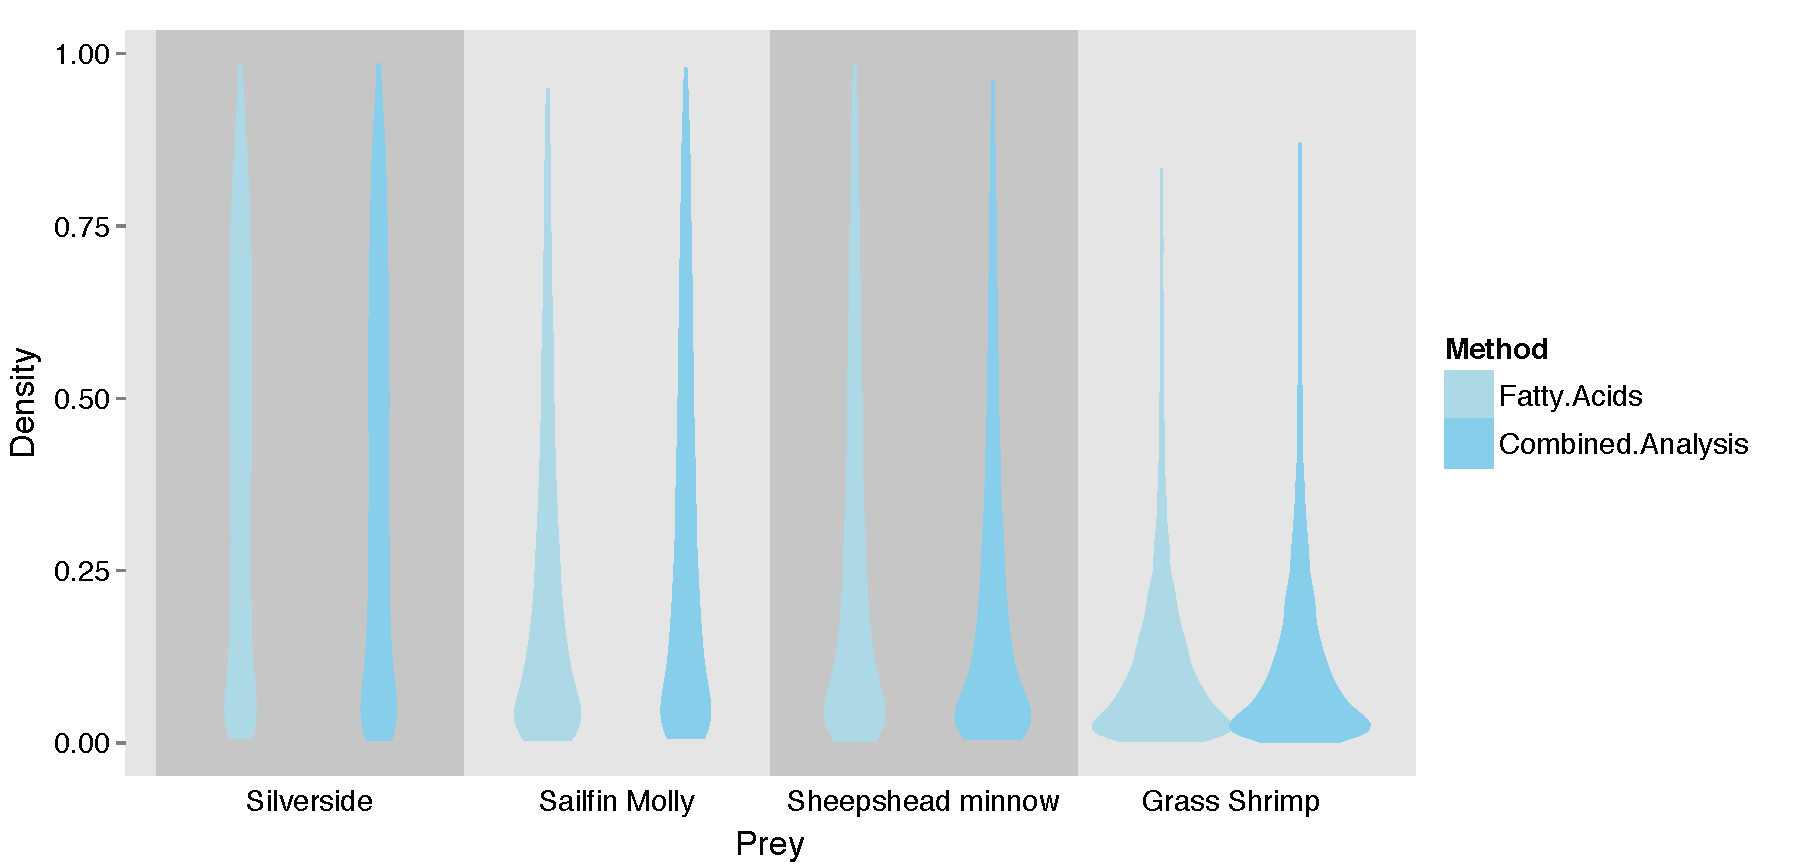
\includegraphics[width=1\textwidth]{figures/SF_comp_plot.pdf}   
    \caption{Posterior densities for diet proportion estimates of SF
      (fish only diet) treatment squid based on FAP and a combined
      (FAP \& SI) analysis. Note that no separate analysis using SI
      only was run.}
    \label{fig:pop_comp_SF}
  \end{center}
\end{figure}

\begin{figure}
  \begin{center}
    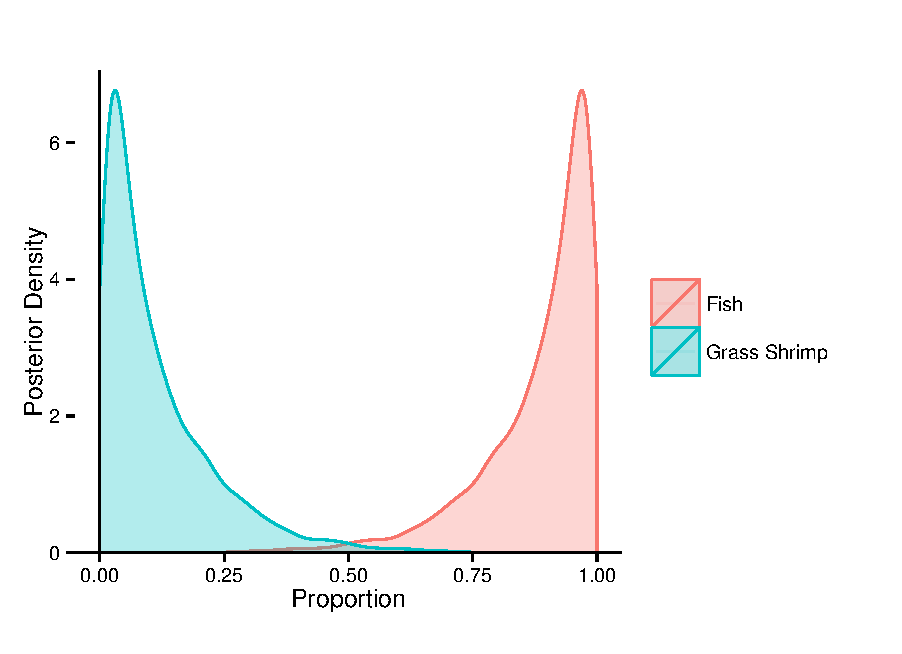
\includegraphics[width=0.65\textwidth]{figures/Fish_plot.pdf}   
    \caption{Posterior densities for diet proportion estimates of SF
      (fish only diet) treatment squid using both SI and FAP,
      combining all fish species into a fish prey group.}
    \label{fig:Fish_plot}
  \end{center}
\end{figure}


%%%%% \begin{figure}
%%%%%   \begin{center}
%%%%%     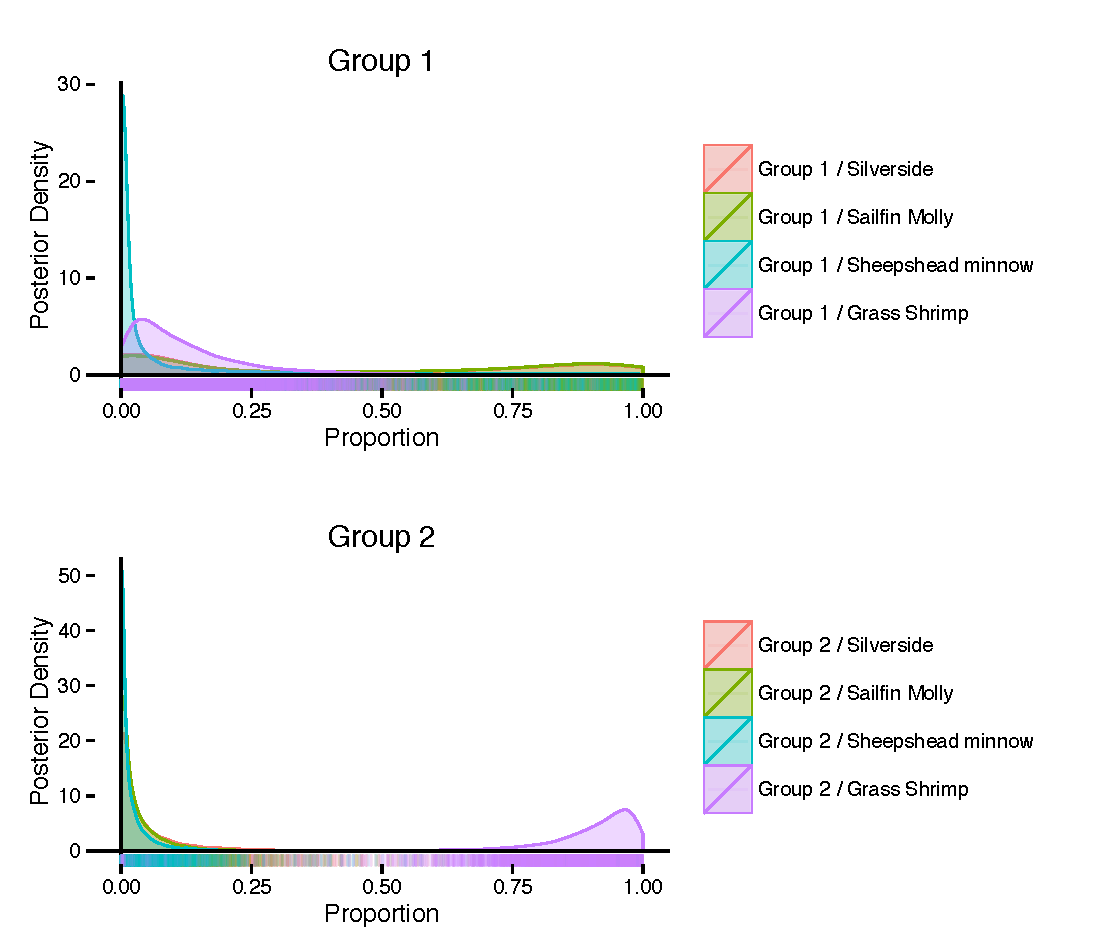
\includegraphics[width=0.75\textwidth]{figures/Group_plot.pdf}   
%%%%%     \caption{Posterior densities for population level diet proportion
%%%%%       estimates of SF (Group 1) and SC (Group 2) squid based on a linear
%%%%%       model for diet proportions using both FAP and SI.}
%%%%%     \label{fig:group_comp}
%%%%%   \end{center}
%%%%% \end{figure}



\section{Discussion}

We presented here a general way to analyse FAP in a Bayesian mixing
model, and demonstrated that the method can be used to estimate diet proportions
in feeding trials while accounting for fatty acid conversion and diet
fat content. The Bayesian framework allows explicit representation of
uncertainty about mixing proportions as a function of uncertainty
about prey distributions, conversion coefficients and fat content,
which represents a substantial improvement over QFASA, the only other
currently available method to analyse diet proportions from FAs.

The general mixing model framework also allowed us to integrate SI and
FAP into a joint model for diet estimation. Both approaches have their
own limits, and the application to squid feeding trials suggests that their combination can substantially reduce uncertainty in diet estimates. As an increasing number of studies combine
these two tracers \citep{tucker_convergence_2008,guest_evidence_2008,guest_trophic_2009,stowasser_experimental_2006,van_der_bank_dietary_2011,jaschinski_carbon_2008},
we suggest that a quantitative method to explicitly compare and combine
markers will allow practitioners to make more robust inference and
explicitly highlight discrepancies among methods that may warrant
future research.

Simulation experiments and sensitivity tests suggested that the mixing model for FAP can
achieve high accuracy of estimated diet proportions in idealized
settings, and the application to squid feeding trials demonstrated the
applicability of the model in a practical, albeit controlled setting. Our results in the
squid study further confirm many of the points made by
\citet{stowasser_experimental_2006}, thereby giving further credibility to our
results. In particular, our analysis of discrimination coefficients
showed that FA in the digestive gland may undergo significant
modification and our analysis of switched diet treatments suggested
that despite the short acclimation time (10-15 days) we can detect
dominant proportions of the switched diet treatments from both SI and
FA. While a complete discussion of these findings is beyond the scope
of this manuscript, these results suggest that the time frame over
which FAP and SI integrate diet proportions in squid is on the order of
weeks rather than months.

Our results from the squid experimental data also showcased the model
sensitivities found using simulated data. Fish species within treatments could
not be discriminated using FAP (and/or SI), and estimated diet
proportions corresponding to fish species in the SF treatment remained
very uncertain. This uncertainty suggests insufficient prey
separation at the species level to accurately estimate diets at the
species level. Despite the uncertainty in estimated diet proportions for
individual fish species, the estimate for the group of all
fish species as opposed to crustacean diets reveals a clear dominance of
fish in the diets (\autoref{fig:Fish_plot}). This example thus illustrates another
benefit of a fully Bayesian treatment: rather than giving
potentially erroneous point estimates in such situations, the wide
95\% intervals suggest that there is insufficient signal in the
data to discriminate among diets at the species level. 

The decrease in accuracy with decreasing source separation reported from simulations and shown in the
squid experiments is thus due to choosing a point estimate within a
large interval rather
than the model suggesting erroneous point estimates of diet proportions. Similarly, for unknown conversion coefficients, posterior
distributions of diet estimates are generally wide, provided that the
prior for conversion coefficients reflects uncertainty. Even when
uncertainty about diet proportions is relatively low, posterior distributions of diet proportions close to 0 or
1 were generally skewed rather than symmetric due to the constrained nature of the diet
proportions, meaning the posterior
mode (the highest posterior probability) is often not located at the
mean of the posterior distribution. In this case, as for very wide and/or flat
posterior distributions, any point estimate
chosen for diet proportions is somewhat arbitrary. Overall estimation error from (posterior mean) point
estimates thus scales with the evenness of the diet proportions as
well as overall uncertainty in diet proportions, and,
rather than relying on point estimates of diet proportions in that case,
it becomes increasingly important to acknowledge uncertainty in the
posterior distributions.

We opted for a fully Bayesian analysis that estimates prey and predator
distributions, as well as individual proportions. However, the Bayesian
approach for FAP comes at a relatively
high computational cost: we found that there are limits to the dimensionality
that the estimation procedure (as we formulated it) can deal with. When working with
fully Bayesian methods in high dimensional applications such as FAP,
where the number of measured variables can be large ($>$20 FAs is common), there
is an inevitable trade-off between computational feasibility and
model dimensionality. Since the model dimensionality depends at once on the number of prey items, predators and
FAs in the analysis, we have found it to be useful to
initially use
predator FAP (geometric) means or relatively few predator signatures to
estimate a single population distribution. Once one has determined
that the model can effectively estimate diet proportions given the
data at hand and knowledge of conversion coefficients, the model can
be re-run with a larger number of predators and/or FAs and, although time consuming, may provide additional
insights. The squid diet example illustrates this strategy: we first
estimated population level parameters for predators (although we used
all predator signatures rather than their geometric mean), and then
proceeded to more complex analyses of individual diet proportions.

To further address the issue of computational complexity, we presented
an approach to variable selection for FAPs. An optimal subset of
variables is usually one that explains the bulk of among prey variance
(represented by CAP axes), but eliminates FAs that only contribute
minimally to separation among sources, and thus only add noise. In our
squid application, we found that retaining only 4 FA was enough to
explain nearly 75\% of among source variance, and adding additional FA
only added a small amount of signal for rapidly increasing
co-linearity in prey signatures. While a limited number of FA may
often be diagnostic of a particular prey type, it may not generally be
the case that a small number of FA account for the bulk of the
signal. The computational cost of high dimensional models in the
Bayesian framework can be limiting in such instances, and the
practical trade-off between model run-time and accuracy of estimated
diet proportions will have to be considered. Our aim is to further
develop the fastinR package to include empirical Bayes options \citep[as
described in][]{parnell_bayesian_2012} that would likely speed up
the models considerably. However, the empirical Bayes approach comes at the cost of considering prey
distribution parameters as known quantities, which may not be desirable with a
small number of prey samples.

Recent developments in SI mixing models have led to increasingly
realistic models in terms of their error structure \citep{hopkins_estimating_2012} and
incorporation of relevant biology, such as time dependent diet
proportions and SI signatures \citep{parnell_bayesian_2012}. Given that our FAP and combined
FAP and SI models employ the same general structure as these models,
such developments are achievable within this framework. It should be
noted, however, that they present the practitioner with requirements for substantial
amounts of data of various kinds (i.e., measurement error estimates,
collection of SI and FAP through time, respectively), and may
substantially increase computational requirements. Nevertheless, we
suggest that the methods presented here provides a basis to use and
combine the two most powerful dietary markers available in
a single framework to produce more robust and comparable diet estimation.

\printbibliography%
\end{flushleft}
\end{spacing}

\end{document}